%----------------------------------------------------------------------------------------
% DE GONIOMETRISCHE CIRKEL EN VERWANTE HOEKEN. Alle opgaven zijn eigen werk.
%
% Opbouw: Probleem, Start, leerstof, en op een nieuwe pagina de Opdrachten en Test jezelf (geen Koppel in de 2de graad).
% Labels van dit hoofdstuk beginnen met h1-.
% Alleen in graden, met hoeken tussen 0 en 360 graden (en negatieve hoeken bij de tegengestelde hoeken).
% Radialen, hoeken groter dan 360 graden en de goniometrische functies komen in de 3de graad.
% Pakket 5: hoeken die 90 graden verschillen (subsectie, voorbeeld, korte oefening) en een opdracht met bewijzen.
%----------------------------------------------------------------------------------------

\mychapter{1}{De goniometrische cirkel}

\begin{probleem}
\vspace{-1mm}\naast{De as van een windturbine staat 80~m boven de grond, en een wiek is 50~m lang. Een wiek start horizontaal, naar rechts, en draait in tegenwijzerzin. Hoe hoog is de punt van de wiek als ze $140^\circ$ gedraaid heeft? En bij welke draaihoeken tussen $0^\circ$ en $360^\circ$ is de punt precies 100~m hoog? Een rechthoekige driehoek met een hoek van $140^\circ$ bestaat niet. Toch geeft je rekenmachine een waarde voor $\sin 140^\circ$. Wat betekent dat getal?}{\begin{tikzpicture}[scale=.034,font=\scriptsize]
  \draw[lijngrijs] (-62,0) -- (62,0);
  \fill[black!12] (-3,0) -- (-1.6,80) -- (1.6,80) -- (3,0) -- cycle;
  \draw[grijs,dashed] (0,80) circle (50);
  \draw[grijs,dashed] (0,80) -- (55,80);
  \draw[accent,line width=1.4pt] (0,80) -- ({50*cos(140)},{80+50*sin(140)});
  \draw[accent!45,line width=1.4pt] (0,80) -- ({50*cos(260)},{80+50*sin(260)}) (0,80) -- ({50*cos(20)},{80+50*sin(20)});
  \draw[->,accent] (12,80) arc[start angle=0,end angle=140,radius=12];
  \node[accent] at (8,98) {$140^\circ$};
  \fill[accent] ({50*cos(140)},{80+50*sin(140)}) circle (40pt) node[above left] {?};
  \fill (0,80) circle (40pt);
  \node[right] at (3,40) {80 m};
  \node[below right] at (22,80) {50 m};
\end{tikzpicture}}
\end{probleem}

\lkr{Leerplan \pakketnaam: LPD 15 (de goniometrische getallen van een hoek op de goniometrische cirkel, verwante hoeken). Het nummer en de afbakening zijn na te kijken in het leerplan. Alles staat in graden. Radialen, hoeken groter dan $360^\circ$ en de grafieken van de goniometrische functies komen pas in de 3de graad, die de goniometrische cirkel opnieuw opbouwt in radialen; dit hoofdstuk legt het fundament en de verwante hoeken in graden.\alleenvoor{5}{ Pakket 5 ziet ook de hoeken die $90^\circ$ verschillen en bewijst identiteiten met verwante hoeken.} Voorkennis uit Driehoeksmeting: sinus, cosinus en tangens in een rechthoekige driehoek, de grondformule, complementaire hoeken en de exacte waarden voor $30^\circ$, $45^\circ$ en $60^\circ$. Laat leerlingen hun rekenmachine in graden zetten (DEG).}

In het handboek Driehoeksmeting waren sinus, cosinus en tangens verhoudingen van zijden in een rechthoekige driehoek. Daar zijn alle hoeken kleiner dan $90^\circ$. Maar een wiek, een wijzer of een rad draait verder, en in een gewone driehoek kan een hoek ook stomp zijn. In dit hoofdstuk breiden we de goniometrische getallen uit tot alle hoeken tussen $0^\circ$ en $360^\circ$, met een cirkel met straal 1: de \emph{goniometrische cirkel}. Daarna zie je hoe hoeken die bij elkaar horen, zoals $40^\circ$ en $140^\circ$, dezelfde goniometrische getallen hebben, op het teken na. In hoofdstuk 2 heb je dat nodig om driehoeken met een stompe hoek te berekenen.

\begin{oefeningen}[Start]
\oef{h1-start-1}

\oef{h1-verken}
\end{oefeningen}

%========================================================================================
\section{Sinus, cosinus en tangens van elke hoek}

\subsection{Hoeken in een assenstelsel}

Een hoek van $140^\circ$ teken je niet in een rechthoekige driehoek, wel in een assenstelsel. Denk aan de wiek uit het probleem: ze vertrekt horizontaal naar rechts, langs de positieve $x$-as, en draait rond de oorsprong. Hoe ver ze gedraaid heeft, is de hoek.

\begin{theorie}
\begin{minipage}[t]{.6\linewidth}
\vspace{0pt}
Een hoek in een assenstelsel heeft zijn hoekpunt in de oorsprong $O$. Het \textbf{\textcolor{accent}{beginbeen}} is de positieve $x$-as. Het \textbf{\textcolor{accent}{eindbeen}} ontstaat door het beginbeen te draaien rond $O$.

\vspace{1mm}
Draai je in \textbf{\textcolor{accent}{tegenwijzerzin}}, dan is de hoek positief. Draai je in \textbf{\textcolor{accent}{wijzerzin}}, dan is de hoek negatief.
\end{minipage}\hfill
\begin{minipage}[t]{.36\linewidth}
\vspace{0pt}
\centering
\begin{tikzpicture}[scale=1.15,font=\scriptsize]
  \draw[->,lijngrijs] (-1.2,0) -- (1.3,0) node[right,text=black] {$x$};
  \draw[->,lijngrijs] (0,-.9) -- (0,1.2) node[above,text=black] {$y$};
  \draw[accent,thick] (0,0) -- (1.1,0) node[above,pos=.78,inner sep=1.5pt] {beginbeen};
  \draw[accent,thick] (0,0) -- (130:1.1) node[above left,inner sep=1pt] {eindbeen};
  \draw[->,accent] (.3,0) arc[start angle=0,end angle=130,radius=.3];
  \node[accent] at (65:.48) {$130^\circ$};
  \draw[->,grijs,dashed] (.55,0) arc[start angle=0,end angle=-50,radius=.55];
  \draw[grijs,dashed] (0,0) -- (-50:1);
  \node[grijs] at (-62:.62) {$-50^\circ$};
\end{tikzpicture}
\end{minipage}
\end{theorie}

\naast{De assen verdelen het vlak in vier \emph{kwadranten}, genummerd in tegenwijzerzin: I rechtsboven, II linksboven, III linksonder en IV rechtsonder. Ligt het eindbeen in het tweede kwadrant, dan zeggen we kort dat de hoek in het tweede kwadrant ligt. Zo liggen de hoeken tussen $90^\circ$ en $180^\circ$ in het tweede kwadrant. Een hoek van $0^\circ$, $90^\circ$, $180^\circ$ of $270^\circ$ ligt op een as, en in geen enkel kwadrant.

Bij een negatieve hoek draai je in wijzerzin. Een hoek van $-50^\circ$ heeft hetzelfde eindbeen als $310^\circ$, want samen met $50^\circ$ maakt $310^\circ$ een volle toer van $360^\circ$.}{\begin{tikzpicture}[scale=1.25,font=\scriptsize]
  \draw[->,lijngrijs] (-1.2,0) -- (1.3,0) node[right,text=black] {$x$};
  \draw[->,lijngrijs] (0,-1.1) -- (0,1.2) node[above,text=black] {$y$};
  \node[align=center] at (.6,.5) {I\\[-1pt]\tiny $0^\circ$ tot $90^\circ$};
  \node[align=center] at (-.6,.5) {II\\[-1pt]\tiny $90^\circ$ tot $180^\circ$};
  \node[align=center] at (-.6,-.5) {III\\[-1pt]\tiny $180^\circ$ tot $270^\circ$};
  \node[align=center] at (.6,-.5) {IV\\[-1pt]\tiny $270^\circ$ tot $360^\circ$};
\end{tikzpicture}}

\voorbeeld{}{Teken de hoek van $230^\circ$ in een assenstelsel. In welk kwadrant ligt hij? Welke negatieve hoek heeft hetzelfde eindbeen?\label{vb:h1-kwadrant}}{%
\uitleg{Na $180^\circ$ wijst het eindbeen naar links. We draaien nog $50^\circ$ verder, naar onder.}
\naast{\begin{stappenvrij}{5.4cm}{5cm}
230^\circ = 180^\circ + 50^\circ & Een halve toer en nog $50^\circ$. \\[1ex]
\text{kwadrant III} & Tussen $180^\circ$ en $270^\circ$. \\[1ex]
230^\circ - 360^\circ = -130^\circ & Een volle toer minder: $130^\circ$ in wijzerzin.
\end{stappenvrij}}{\begin{tikzpicture}[scale=1.1,font=\scriptsize]
  \draw[->,lijngrijs] (-1.2,0) -- (1.3,0) node[right,text=black] {$x$};
  \draw[->,lijngrijs] (0,-1.2) -- (0,1.2) node[above,text=black] {$y$};
  \draw[accent,thick] (0,0) -- (230:1.15);
  \draw[->,accent] (.25,0) arc[start angle=0,end angle=230,radius=.25];
  \draw[->,grijs,dashed] (.65,0) arc[start angle=0,end angle=-130,radius=.65];
  \node[accent,fill=white,inner sep=1pt] at (100:.48) {$230^\circ$};
  \node[grijs] at (-40:.95) {$-130^\circ$};
\end{tikzpicture}}}

\begin{oefeningen}
\oef{h1-kwadrant}
\end{oefeningen}

\subsection{Sinus en cosinus}

Hoe geef je een hoek als $140^\circ$ een sinus? Kijk eerst naar een scherpe hoek. In de Verken vond je dat de coördinaten van het punt bij $30^\circ$, gedeeld door de straal, precies $\cos 30^\circ$ en $\sin 30^\circ$ zijn. Kies je de straal 1, dan hoef je zelfs niet meer te delen.

\naast{Neem een cirkel met middelpunt $O$ en straal 1, en een scherpe hoek $\alpha$. Het eindbeen snijdt de cirkel in het punt $P$. De loodlijn uit $P$ op de $x$-as maakt een rechthoekige driehoek met schuine zijde $\lengte{OP} = 1$. De aanliggende rechthoekszijde is $x_P$, de overstaande is $y_P$. Dus
\[\cos\alpha = \frac{x_P}{1} = x_P \qquad \text{en} \qquad \sin\alpha = \frac{y_P}{1} = y_P .\]
Voor een scherpe hoek is de cosinus dus de $x$-coördinaat van $P$ en de sinus de $y$-coördinaat. Dat idee werkt voor elke hoek, ook als er geen driehoek meer is. Daarom nemen we het als definitie.}{\begin{tikzpicture}[scale=1.55,font=\scriptsize]
  \gonicirkel[t]
  \fill[accent!12] (0,0) -- ({cos(35)},0) -- (35:1) -- cycle;
  \draw[accent] ({cos(35)},0) -- (35:1);
  \gonipunt{35}{P}{above right}
  \node[accent] at (17:.38) {$\alpha$};
  \node[above left,inner sep=1pt] at (35:.6) {$1$};
  \node[below] at ({cos(35)/2},0) {$x_P$};
  \node[right] at ({cos(35)},{sin(35)/2}) {$y_P$};
\end{tikzpicture}}

\begin{theorie}
\begin{minipage}[t]{.6\linewidth}
\vspace{0pt}
De \textbf{\textcolor{accent}{goniometrische cirkel}} is de cirkel met middelpunt $O(0, 0)$ en straal 1. Het eindbeen van een hoek $\alpha$ snijdt die cirkel in het punt $P$. Dan is

\vspace{1mm}
\qquad $\formule{\cos\alpha = x_P} \qquad \text{en} \qquad \formule{\sin\alpha = y_P}$

\vspace{1mm}
zodat $P$ het punt $(\cos\alpha, \sin\alpha)$ is.
\end{minipage}\hfill
\begin{minipage}[t]{.36\linewidth}
\vspace{0pt}
\centering
\begin{tikzpicture}[scale=1.35,font=\scriptsize]
  \gonicirkel
  \draw[accent,dashed] (140:1) -- ({cos(140)},0);
  \draw[accent,dashed] (140:1) -- (0,{sin(140)});
  \gonipunt{140}{P}{above left}
  \node[accent] at (70:.38) {$\alpha$};
  \node[below] at ({cos(140)},0) {$\cos\alpha$};
  \node[right] at (0,{sin(140)}) {$\sin\alpha$};
\end{tikzpicture}
\end{minipage}
\end{theorie}

Voor een scherpe hoek geeft dat dezelfde sinus en cosinus als in een rechthoekige driehoek: er verandert niets aan wat je al kende. Nieuw is dat een cosinus of een sinus nu ook negatief of nul kan zijn. Omdat $P$ op een cirkel met straal 1 ligt, liggen de sinus en de cosinus altijd tussen $-1$ en $1$. De punten op de cirkel heten ook de \emph{beeldpunten} van de hoeken.

\voorbeeld{}{Schat $\cos 140^\circ$ en $\sin 140^\circ$ met een tekening op de goniometrische cirkel. Controleer met de rekenmachine.\label{vb:h1-140}}{%
\uitleg{We tekenen het punt $P$ bij $140^\circ$ op een cirkel met straal 1 op ruitjespapier (10 ruitjes voor 1), en lezen de coördinaten af.}
\naast{\begin{stappenvrij}{5.6cm}{4.6cm}
P \approx (-0{,}77;\ 0{,}64) & Afgelezen op de figuur. \\[1ex]
\cos 140^\circ \approx -0{,}7660 & De $x$-coördinaat, negatief: $P$ ligt links van de $y$-as. \\[1ex]
\sin 140^\circ \approx 0{,}6428 & De $y$-coördinaat, positief: $P$ ligt boven de $x$-as.
\end{stappenvrij}}{\begin{tikzpicture}[scale=1.5,font=\scriptsize]
  \draw[black!14,very thin,step=.1] (-1.05,-.25) grid (1.05,1.05);
  \draw[->,lijngrijs] (-1.15,0) -- (1.2,0) node[right,text=black] {$x$};
  \draw[->,lijngrijs] (0,-.25) -- (0,1.15) node[above,text=black] {$y$};
  \draw[grijs] (1,0) arc[start angle=0,end angle=180,radius=1];
  \draw[accent,dashed] (140:1) -- ({cos(140)},0);
  \draw[accent,dashed] (140:1) -- (0,{sin(140)});
  \gonipunt{140}{P}{above left}
  \node[below,inner sep=1pt] at ({cos(140)},0) {\tiny $-0{,}77$};
  \node[right,inner sep=1pt] at (0,{sin(140)+.07}) {\tiny $0{,}64$};
  \node[below,inner sep=1pt] at (1,0) {\tiny $1$};
\end{tikzpicture}}
Dit is de hoek van de voorkant van dit boek. De rekenmachine geeft dezelfde waarden, met meer decimalen: ze rekent op de goniometrische cirkel.}

Bij de hoeken op de assen ligt $P$ op een van de vier snijpunten van de cirkel met de assen. Daar lees je de sinus en de cosinus meteen af.

\voorbeeld{}{Geef de sinus en de cosinus van $0^\circ$, $90^\circ$, $180^\circ$ en $270^\circ$.\label{vb:h1-assen}}{%
\uitleg{We zoeken telkens het punt $P$ op de cirkel: rechts, boven, links of onder. Zijn coördinaten zijn de cosinus en de sinus.}
\naast{\renewcommand{\arraystretch}{1.3}%
\begin{tabular}{|c|c|c|c|c|}
\hline
$\alpha$ & $0^\circ$ & $90^\circ$ & $180^\circ$ & $270^\circ$ \\ \hline
$P$ & $(1, 0)$ & $(0, 1)$ & $(-1, 0)$ & $(0, -1)$ \\ \hline
$\cos\alpha$ & $1$ & $0$ & $-1$ & $0$ \\ \hline
$\sin\alpha$ & $0$ & $1$ & $0$ & $-1$ \\ \hline
\end{tabular}}{\begin{tikzpicture}[scale=.85,font=\scriptsize]
  \gonicirkel
  \foreach \h/\n/\p in {0/0^\circ/below right,90/90^\circ/above left,180/180^\circ/below left,270/270^\circ/below left}{
    \fill[accent] (\h:1) circle (.05) node[\p,inner sep=1pt] {$\n$};}
\end{tikzpicture}}
Je hoeft de tabel niet van buiten te leren: met een schets van de cirkel vind je ze altijd terug.}

\begin{oefeningen}
\oef{h1-sincos}
\end{oefeningen}

\subsection{Een cirkel met een andere straal}

Voor de wiek uit het probleem is de straal niet 1, maar 50~m. Een cirkel met straal $r$ is een vergroting van de goniometrische cirkel met factor $r$, vanuit $O$. Bij die vergroting worden beide coördinaten van $P$ met $r$ vermenigvuldigd.

\begin{theorie}
\begin{stelling}{Punt op een cirkel met straal $r$}
Het punt op afstand $r$ van $O$, op het eindbeen van de hoek $\alpha$, heeft coördinaten

\vspace{1mm}
\qquad $\formule{(r\cos\alpha,\ r\sin\alpha)}$
\end{stelling}
\end{theorie}

\voorbeeld{}{De arm van een robot is 60~cm lang en draait rond een as in de oorsprong. Hij vertrekt horizontaal naar rechts en draait $115^\circ$ in tegenwijzerzin. Waar is het uiteinde van de arm? Rond af op een millimeter.\label{vb:h1-straal}}{%
\uitleg{Het uiteinde ligt op een cirkel met straal 60, op het eindbeen van $115^\circ$. We vermenigvuldigen de cosinus en de sinus met 60.}
\naast{\begin{stappenvrij}{5.4cm}{5cm}
x = 60 \cos 115^\circ \approx -25{,}36 & Negatief: links van de as. \\[1ex]
y = 60 \sin 115^\circ \approx 54{,}38 & Positief: boven de as.
\end{stappenvrij}}{\begin{tikzpicture}[scale=.022,font=\scriptsize]
  \draw[->,lijngrijs] (-50,0) -- (70,0) node[right,text=black] {$x$};
  \draw[->,lijngrijs] (0,-8) -- (0,70) node[above,text=black] {$y$};
  \draw[grijs,dashed] (60,0) arc[start angle=0,end angle=180,radius=60];
  \draw[accent,line width=1.5pt] (0,0) -- (115:60);
  \draw[->,accent] (15,0) arc[start angle=0,end angle=115,radius=15];
  \node[accent] at (40:26) {$115^\circ$};
  \fill[accent] (115:60) circle (70pt);
  \draw[accent,dashed] (115:60) -- ({60*cos(115)},0);
\end{tikzpicture}}
Het uiteinde is ongeveer 25,4~cm links van de as en 54,4~cm hoger.}

%----------------------------------------------------------------------------------------
\subsection{De tangens}

In een rechthoekige driehoek bewees je dat $\tan\alpha = \frac{\sin\alpha}{\cos\alpha}$. Die formule gebruiken we nu als definitie voor elke hoek.

\begin{theorie}
De \textbf{\textcolor{accent}{tangens}} van een hoek $\alpha$ met $\cos\alpha \neq 0$ is

\vspace{1mm}
\qquad $\formule{\tan\alpha = \frac{\sin\alpha}{\cos\alpha}}$
\end{theorie}

\naast{Voor $90^\circ$ en $270^\circ$ is de cosinus 0: daar bestaat de tangens niet. Meetkundig is $\tan\alpha = \frac{y_P}{x_P}$ de richtingscoëfficiënt van de rechte $OP$. Die rechte snijdt de verticale raaklijn aan de cirkel in $(1, 0)$ in het punt $T(1, \tan\alpha)$, want op die rechte stijg je $\tan\alpha$ per stap 1 naar rechts. Zo kun je de tangens ook op de figuur aflezen. Daar komt de naam vandaan: \textit{tangens} is Latijn voor \textit{rakend}. Staat $OP$ verticaal, dan snijdt ze de raaklijn niet, en bestaat de tangens niet.}{\begin{tikzpicture}[scale=1.3,font=\scriptsize]
  \gonicirkel
  \draw[grijs] (1,-1.25) -- (1,1.35);
  \draw[accent,thick] (0,0) -- (1,{tan(40)});
  \fill[accent] (40:1) circle (.035) node[above left] {$P$};
  \fill[accent] (1,{tan(40)}) circle (.035) node[right] {$T$};
  \draw[->,accent] (.24,0) arc[start angle=0,end angle=40,radius=.24];
  \node[accent] at (20:.36) {$\alpha$};
  \draw[decorate,decoration={brace,amplitude=3pt,mirror}] (1.05,0) -- (1.05,{tan(40)}) node[midway,right=2pt] {$\tan\alpha$};
\end{tikzpicture}}

\voorbeeld{}{Bereken $\tan 140^\circ$ uit de sinus en de cosinus, en controleer met de rekenmachine. Wat betekent het teken?\label{vb:h1-tan}}{%
\uitleg{We delen de sinus door de cosinus uit voorbeeld \ref{vb:h1-140}. Een positief getal gedeeld door een negatief getal is negatief.}
\begin{stappen}
\tan 140^\circ = \dfrac{\sin 140^\circ}{\cos 140^\circ} \approx \dfrac{0{,}6428}{-0{,}7660} \approx -0{,}8391 & De definitie. De rekenmachine geeft hetzelfde.
\end{stappen}
De rechte $OP$ daalt: wie naar rechts gaat, gaat naar beneden. Haar richtingscoëfficiënt is negatief.}

\begin{oefeningen}
\oef{h1-tan}
\end{oefeningen}

\subsection{Het teken in elk kwadrant}

Of een sinus of cosinus positief of negatief is, zie je aan de plaats van $P$. In het tweede kwadrant ligt $P$ links van de $y$-as en boven de $x$-as: de cosinus is negatief, de sinus positief, en de tangens als quotiënt dus negatief. Zo vind je het teken in elk kwadrant.

\begin{theorie}
\begin{minipage}[t]{.56\linewidth}
\vspace{0pt}
Het teken van de goniometrische getallen in elk kwadrant:

\vspace{2mm}
\centering
\renewcommand{\arraystretch}{1.35}
\begin{tabular}{|c|c|c|c|c|}
\hline
kwadrant & I & II & III & IV \\ \hline
$\sin\alpha$ & $\formule{+}$ & $\formule{+}$ & $\formule{-}$ & $\formule{-}$ \\ \hline
$\cos\alpha$ & $\formule{+}$ & $\formule{-}$ & $\formule{-}$ & $\formule{+}$ \\ \hline
$\tan\alpha$ & $\formule{+}$ & $\formule{-}$ & $\formule{+}$ & $\formule{-}$ \\ \hline
\end{tabular}
\end{minipage}\hfill
\begin{minipage}[t]{.4\linewidth}
\vspace{0pt}
\centering
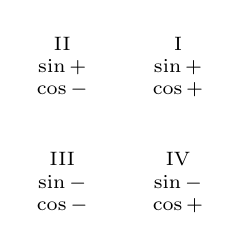
\begin{tikzpicture}[scale=1.75,font=\scriptsize]
  \gonicirkel
  \node[align=center] at (.42,.42) {I\\$\sin +$\\$\cos +$};
  \node[align=center] at (-.42,.42) {II\\$\sin +$\\$\cos -$};
  \node[align=center] at (-.42,-.42) {III\\$\sin -$\\$\cos -$};
  \node[align=center] at (.42,-.42) {IV\\$\sin -$\\$\cos +$};
\end{tikzpicture}
\end{minipage}
\end{theorie}

De tabel moet je niet van buiten leren: een schets van de cirkel volstaat. De sinus is positief boven de $x$-as, de cosinus rechts van de $y$-as. De tangens is positief als sinus en cosinus hetzelfde teken hebben.

\voorbeeld{}{Bepaal zonder rekenmachine het teken van $\sin 200^\circ$, $\cos 200^\circ$ en $\tan 200^\circ$.\label{vb:h1-teken}}{%
\uitleg{We zoeken eerst het kwadrant. Daarna lezen we het teken af aan de plaats van $P$.}
\begin{stappen}
180^\circ < 200^\circ < 270^\circ & De hoek ligt in het derde kwadrant. \\[1ex]
\sin 200^\circ < 0 \quad\text{en}\quad \cos 200^\circ < 0 & $P$ ligt links onder: beide coördinaten zijn negatief. \\[1ex]
\tan 200^\circ > 0 & Negatief gedeeld door negatief is positief.
\end{stappen}
Controle met de rekenmachine: $\sin 200^\circ \approx -0{,}3420$, $\cos 200^\circ \approx -0{,}9397$ en $\tan 200^\circ \approx 0{,}3640$.}

\begin{oefeningen}
\oef{h1-teken}
\end{oefeningen}

\subsection{De grondformule voor elke hoek}

Voor een scherpe hoek is $\sin^2\alpha + \cos^2\alpha = 1$ de stelling van Pythagoras. Geldt dat nog voor $140^\circ$? Met de rekenmachine: $0{,}6428^2 + ({-0{,}7660})^2 = 0{,}4132 + 0{,}5868 = 1$. Op de goniometrische cirkel zie je waarom.

\begin{theorie}
\begin{minipage}[t]{.64\linewidth}
\vspace{0pt}
\begin{stelling}{Grondformule}
Voor elke hoek $\alpha$ geldt

\vspace{1mm}
\qquad $\formule{\sin^2\alpha + \cos^2\alpha = 1}$
\end{stelling}

\begin{bewijs}
Ligt $P(\cos\alpha, \sin\alpha)$ niet op een as, dan maakt de loodlijn uit $P$ op de $x$-as een rechthoekige driehoek met rechthoekszijden $\abs{\cos\alpha}$ en $\abs{\sin\alpha}$ en schuine zijde $\lengte{OP} = 1$. Volgens Pythagoras is
\bewijsregel{\abs{\cos\alpha}^2 + \abs{\sin\alpha}^2 = 1 , \quad \text{dus} \quad \cos^2\alpha + \sin^2\alpha = 1 ,}
want een getal en zijn absolute waarde hebben hetzelfde kwadraat. Ligt $P$ op een as, dan is een van de twee getallen 0 en het andere $1$ of $-1$, en klopt de formule ook.
\end{bewijs}
\end{minipage}\hfill
\begin{minipage}[t]{.32\linewidth}
\vspace{2mm}
\centering
\begin{tikzpicture}[scale=1.25,font=\scriptsize]
  \gonicirkel
  \fill[accent!12] (0,0) -- ({cos(140)},0) -- (140:1) -- cycle;
  \draw[accent] ({cos(140)},0) -- (140:1);
  \gonipunt{140}{P}{above left}
  \node[below] at ({cos(140)/2},0) {$\abs{\cos\alpha}$};
  \node[left] at ({cos(140)},{sin(140)/2}) {$\abs{\sin\alpha}$};
\end{tikzpicture}
\end{minipage}
\end{theorie}

Ken je de sinus van een hoek, dan geeft de grondformule de cosinus op het teken na: er zijn twee getallen met hetzelfde kwadraat. Het kwadrant beslist welk teken het wordt.

\voorbeeld{}{Van een hoek $\alpha$ in het derde kwadrant is $\cos\alpha = -\tfrac{5}{13}$. Bereken exact $\sin\alpha$ en $\tan\alpha$.\label{vb:h1-grond}}{%
\uitleg{De grondformule geeft $\sin^2\alpha$. In het derde kwadrant ligt $P$ onder de $x$-as, dus de sinus is negatief.}
\begin{stappen}
\sin^2\alpha = 1 - \tfrac{25}{169} = \tfrac{144}{169} & Grondformule. \\[1ex]
\sin\alpha = -\tfrac{12}{13} & Niet $+\tfrac{12}{13}$: in het derde kwadrant is de sinus negatief. \\[1ex]
\tan\alpha = \dfrac{-12/13}{-5/13} = \tfrac{12}{5} & Sinus gedeeld door cosinus; positief in het derde kwadrant.
\end{stappen}}

\begin{werkwijze}
Bereken het kwadraat van het ontbrekende getal met de grondformule, en neem de vierkantswortel. Kies het teken met het kwadrant: de sinus is positief boven de $x$-as, de cosinus rechts van de $y$-as. Bereken daarna de tangens als quotiënt.
\end{werkwijze}

\nujij{Van een hoek $\alpha$ in het vierde kwadrant is $\cos\alpha = 0{,}8$. Bereken $\sin\alpha$ en $\tan\alpha$.}{$\sin^2\alpha = 1 - 0{,}64 = 0{,}36$, en in het vierde kwadrant is de sinus negatief: $\sin\alpha = -0{,}6$ en $\tan\alpha = -0{,}75$.}

\begin{oefeningen}
\oef{h1-grond}
\end{oefeningen}

%========================================================================================
\section{Verwante hoeken}

In de Verken vond je voor $30^\circ$, $150^\circ$, $210^\circ$ en $330^\circ$ vier punten met dezelfde coördinaten, op het teken na. Dat komt doordat een cirkel zo symmetrisch is: spiegel je $P$ om een as of om $O$, dan kom je weer op de cirkel uit, bij een andere hoek. Zulke hoeken heten \emph{verwante hoeken}. Ken je de goniometrische getallen van één hoek, dan ken je ze ook van zijn verwante hoeken.

\figuren{\begin{tikzpicture}[scale=1.3,font=\scriptsize]
  \gonicirkel
  \foreach \h/\n/\p in {35/\alpha/right,145/180^\circ - \alpha/left,215/180^\circ + \alpha/left,-35/-\alpha/right}{
    \draw[accent] (0,0) -- (\h:1);
    \fill[accent] (\h:1) circle (.035) node[\p] {$\n$};}
  \draw[accent,dashed] (35:1) -- (145:1) (35:1) -- (-35:1) (35:1) -- (215:1);
\end{tikzpicture}\hspace{1.5cm}
\begin{tikzpicture}[scale=1.3,font=\scriptsize]
  \gonicirkel
  \draw[grijs,dashed] (-1.1,-1.1) -- (1.2,1.2) node[above right] {$y = x$};
  \foreach \h/\n/\p in {25/\alpha/right,65/90^\circ - \alpha/above right}{
    \draw[accent] (0,0) -- (\h:1);
    \fill[accent] (\h:1) circle (.035) node[\p] {$\n$};}
  \draw[accent,dashed] (25:1) -- (65:1);
\end{tikzpicture}}

We bekijken ze een voor een: telkens een spiegeling, en wat die met de coördinaten van $P$ doet.

\subsection{Supplementaire hoeken}

Twee hoeken zijn \emph{supplementair} als ze samen $180^\circ$ zijn, zoals $40^\circ$ en $140^\circ$. Teken de punten bij $40^\circ$ en $140^\circ$: ze liggen even hoog, en even ver van de $y$-as, maar aan de andere kant. Ze zijn elkaars spiegelbeeld om de $y$-as.

\begin{theorie}
\begin{minipage}[t]{.64\linewidth}
\vspace{0pt}
\begin{stelling}{Supplementaire hoeken}
Voor elke hoek $\alpha$ geldt

\vspace{1mm}
\qquad $\formule{\sin(180^\circ - \alpha) = \sin\alpha}$

\qquad $\formule{\cos(180^\circ - \alpha) = -\cos\alpha}$

\qquad $\formule{\tan(180^\circ - \alpha) = -\tan\alpha}$ \quad (als $\cos\alpha \neq 0$)
\end{stelling}

\begin{bewijs}
Spiegel $P$ om de $y$-as. Het beeld $P'$ ligt op de cirkel, en $OP'$ maakt met de negatieve $x$-as dezelfde hoek als $OP$ met de positieve $x$-as. Dus hoort $P'$ bij de hoek $180^\circ - \alpha$. Die spiegeling behoudt de $y$-coördinaat en verandert het teken van de $x$-coördinaat:
\bewijsregel{P'\bigl(\cos(180^\circ - \alpha), \sin(180^\circ - \alpha)\bigr) = P'(-\cos\alpha, \sin\alpha) .}
Delen geeft $\tan(180^\circ - \alpha) = \dfrac{\sin\alpha}{-\cos\alpha} = -\tan\alpha$.
\end{bewijs}
\end{minipage}\hfill
\begin{minipage}[t]{.32\linewidth}
\vspace{3mm}
\centering
\begin{tikzpicture}[scale=1.3,font=\scriptsize]
  \gonicirkel
  \draw[accent] (0,0) -- (40:1) (0,0) -- (140:1);
  \draw[accent,dashed] (40:1) -- (140:1);
  \fill[accent] (40:1) circle (.035) node[above right] {$P$};
  \fill[accent] (140:1) circle (.035) node[above left] {$P'$};
  \draw[accent] (.25,0) arc[start angle=0,end angle=40,radius=.25];
  \draw[accent] (-.25,0) arc[start angle=180,end angle=140,radius=.25];
  \node[accent] at (20:.4) {$\alpha$};
  \node[accent] at (160:.4) {$\alpha$};
\end{tikzpicture}
\end{minipage}
\end{theorie}

Supplementaire hoeken hebben dus dezelfde sinus, en een tegengestelde cosinus en tangens. Dat is belangrijk voor driehoeken: een stompe hoek van een driehoek heeft dezelfde sinus als de scherpe hoek die hem tot $180^\circ$ aanvult.

\voorbeeld{}{Bereken exact $\sin 120^\circ$, $\cos 120^\circ$ en $\tan 120^\circ$.\label{vb:h1-suppl}}{%
\uitleg{$120^\circ = 180^\circ - 60^\circ$: een supplementaire hoek van $60^\circ$, waarvan we de exacte waarden kennen. $P$ ligt in het tweede kwadrant.}
\begin{stappen}
\sin 120^\circ = \sin(180^\circ - 60^\circ) = \sin 60^\circ = \tfrac{\sqrt3}{2} & Supplementaire hoeken: dezelfde sinus. \\[1ex]
\cos 120^\circ = -\cos 60^\circ = -\tfrac12 & Tegengestelde cosinus. \\[1ex]
\tan 120^\circ = -\tan 60^\circ = -\sqrt3 & Tegengestelde tangens.
\end{stappen}
Controle met het kwadrant: in het tweede kwadrant is de sinus positief en zijn cosinus en tangens negatief.}

\begin{oefeningen}
\oef{h1-suppl}
\end{oefeningen}

\subsection{Antisupplementaire hoeken}

De hoeken $\alpha$ en $180^\circ + \alpha$ verschillen een halve toer. Ze heten \emph{antisupplementair}. Hun punten liggen diametraal tegenover elkaar: ze zijn elkaars spiegelbeeld om de oorsprong.

\begin{theorie}
\begin{minipage}[t]{.64\linewidth}
\vspace{0pt}
\begin{stelling}{Antisupplementaire hoeken}
Voor elke hoek $\alpha$ geldt

\vspace{1mm}
\qquad $\formule{\sin(180^\circ + \alpha) = -\sin\alpha}$

\qquad $\formule{\cos(180^\circ + \alpha) = -\cos\alpha}$

\qquad $\formule{\tan(180^\circ + \alpha) = \tan\alpha}$ \quad (als $\cos\alpha \neq 0$)
\end{stelling}

\begin{bewijs}
Draai je $OP$ nog $180^\circ$ verder, dan kom je in het punt $P'$ dat diametraal tegenover $P$ ligt: het spiegelbeeld van $P$ om $O$. Die spiegeling verandert het teken van beide coördinaten:
\bewijsregel{P'\bigl(\cos(180^\circ + \alpha), \sin(180^\circ + \alpha)\bigr) = P'(-\cos\alpha, -\sin\alpha) .}
Delen geeft $\tan(180^\circ + \alpha) = \dfrac{-\sin\alpha}{-\cos\alpha} = \tan\alpha$.
\end{bewijs}
\end{minipage}\hfill
\begin{minipage}[t]{.32\linewidth}
\vspace{3mm}
\centering
\begin{tikzpicture}[scale=1.3,font=\scriptsize]
  \gonicirkel
  \draw[accent] (220:1) -- (40:1);
  \fill[accent] (40:1) circle (.035) node[above right] {$P$};
  \fill[accent] (220:1) circle (.035) node[below left] {$P'$};
  \draw[accent] (.25,0) arc[start angle=0,end angle=40,radius=.25];
  \draw[accent] (-.25,0) arc[start angle=180,end angle=220,radius=.25];
  \node[accent] at (20:.4) {$\alpha$};
  \node[accent] at (200:.4) {$\alpha$};
\end{tikzpicture}
\end{minipage}
\end{theorie}

Een halve toer verder keren de sinus en de cosinus allebei van teken. Hun quotiënt, de tangens, blijft dan gelijk.

\voorbeeld{}{Bereken exact $\sin 225^\circ$, $\cos 225^\circ$ en $\tan 225^\circ$.\label{vb:h1-anti}}{%
\uitleg{$225^\circ = 180^\circ + 45^\circ$: een antisupplementaire hoek van $45^\circ$. $P$ ligt in het derde kwadrant.}
\begin{stappen}
\sin 225^\circ = -\sin 45^\circ = -\tfrac{\sqrt2}{2} & Antisupplementair: tegengestelde sinus. \\[1ex]
\cos 225^\circ = -\cos 45^\circ = -\tfrac{\sqrt2}{2} & Tegengestelde cosinus. \\[1ex]
\tan 225^\circ = \tan 45^\circ = 1 & Dezelfde tangens.
\end{stappen}}

\begin{oefeningen}
\oef{h1-anti}
\end{oefeningen}

\subsection{Tegengestelde hoeken}

De hoeken $\alpha$ en $-\alpha$ draaien even ver, maar in tegengestelde zin. Ze heten \emph{tegengestelde hoeken}. Hun punten zijn elkaars spiegelbeeld om de $x$-as. De hoek $-\alpha$ heeft hetzelfde eindbeen als $360^\circ - \alpha$: zo kun je ook met positieve hoeken werken.

\begin{theorie}
\begin{minipage}[t]{.64\linewidth}
\vspace{0pt}
\begin{stelling}{Tegengestelde hoeken}
Voor elke hoek $\alpha$ geldt

\vspace{1mm}
\qquad $\formule{\sin(-\alpha) = -\sin\alpha}$

\qquad $\formule{\cos(-\alpha) = \cos\alpha}$

\qquad $\formule{\tan(-\alpha) = -\tan\alpha}$ \quad (als $\cos\alpha \neq 0$)

\vspace{1mm}
en hetzelfde voor $360^\circ - \alpha$ in plaats van $-\alpha$.
\end{stelling}

\begin{bewijs}
Spiegel $P$ om de $x$-as. Het beeld $P'$ ligt op de cirkel, en $OP'$ maakt dezelfde hoek met de $x$-as, maar aan de andere kant: $P'$ hoort bij $-\alpha$. Die spiegeling behoudt de $x$-coördinaat en verandert het teken van de $y$-coördinaat:
\bewijsregel{P'\bigl(\cos(-\alpha), \sin(-\alpha)\bigr) = P'(\cos\alpha, -\sin\alpha) .}
Delen geeft $\tan(-\alpha) = -\tan\alpha$. De hoek $360^\circ - \alpha$ hoort bij hetzelfde punt $P'$, en heeft dus dezelfde goniometrische getallen als $-\alpha$.
\end{bewijs}
\end{minipage}\hfill
\begin{minipage}[t]{.32\linewidth}
\vspace{3mm}
\centering
\begin{tikzpicture}[scale=1.3,font=\scriptsize]
  \gonicirkel
  \draw[accent] (0,0) -- (40:1) (0,0) -- (-40:1);
  \draw[accent,dashed] (40:1) -- (-40:1);
  \fill[accent] (40:1) circle (.035) node[above right] {$P$};
  \fill[accent] (-40:1) circle (.035) node[below right] {$P'$};
  \draw[->,accent] (.25,0) arc[start angle=0,end angle=40,radius=.25];
  \draw[->,accent] (.25,0) arc[start angle=0,end angle=-40,radius=.25];
  \node[accent] at (20:.42) {$\alpha$};
  \node[accent] at (-20:.48) {$-\alpha$};
\end{tikzpicture}
\end{minipage}
\end{theorie}

De cosinus merkt niets van het teken van de hoek, de sinus en de tangens wel.

\voorbeeld{}{Bereken exact $\sin 300^\circ$, $\cos 300^\circ$ en $\tan 300^\circ$.\label{vb:h1-tegen}}{%
\uitleg{$300^\circ = 360^\circ - 60^\circ$: dat punt hoort ook bij $-60^\circ$, het tegengestelde van $60^\circ$. $P$ ligt in het vierde kwadrant.}
\begin{stappen}
\sin 300^\circ = \sin(-60^\circ) = -\sin 60^\circ = -\tfrac{\sqrt3}{2} & Tegengestelde hoeken: tegengestelde sinus. \\[1ex]
\cos 300^\circ = \cos 60^\circ = \tfrac12 & Dezelfde cosinus. \\[1ex]
\tan 300^\circ = -\tan 60^\circ = -\sqrt3 & Tegengestelde tangens.
\end{stappen}
Controle met het kwadrant: in het vierde kwadrant is alleen de cosinus positief.}

\begin{oefeningen}
\oef{h1-tegen}
\end{oefeningen}

\subsection{Complementaire hoeken}

In Driehoeksmeting zag je dat de twee scherpe hoeken van een rechthoekige driehoek samen $90^\circ$ zijn, en dat $\sin(90^\circ - \alpha) = \cos\alpha$. Twee hoeken met som $90^\circ$ heten \emph{complementair}. Op de goniometrische cirkel zijn hun punten elkaars spiegelbeeld om de rechte $y = x$, en zo geldt de eigenschap voor elke hoek, niet alleen voor scherpe hoeken.

\begin{theorie}
\begin{minipage}[t]{.64\linewidth}
\vspace{0pt}
\begin{stelling}{Complementaire hoeken}
Voor elke hoek $\alpha$ geldt

\vspace{1mm}
\qquad $\formule{\sin(90^\circ - \alpha) = \cos\alpha}$

\qquad $\formule{\cos(90^\circ - \alpha) = \sin\alpha}$

\qquad $\formule{\tan(90^\circ - \alpha) = \frac{1}{\tan\alpha}}$

\vspace{1mm}
de laatste als $\sin\alpha \neq 0$ en $\cos\alpha \neq 0$.
\end{stelling}

\begin{bewijs}
Spiegel $P$ om de rechte $y = x$. Die spiegeling wisselt de $x$- en de $y$-coördinaat om, en brengt de positieve $x$-as naar de positieve $y$-as. $OP'$ maakt dus met de $y$-as de hoek $\alpha$, en met de $x$-as de hoek $90^\circ - \alpha$:
\bewijsregel{P'\bigl(\cos(90^\circ - \alpha), \sin(90^\circ - \alpha)\bigr) = P'(\sin\alpha, \cos\alpha) .}
Delen geeft $\tan(90^\circ - \alpha) = \dfrac{\cos\alpha}{\sin\alpha} = \dfrac{1}{\tan\alpha}$.
\end{bewijs}
\end{minipage}\hfill
\begin{minipage}[t]{.32\linewidth}
\vspace{3mm}
\centering
\begin{tikzpicture}[scale=1.3,font=\scriptsize]
  \gonicirkel
  \draw[grijs,dashed] (-.9,-.9) -- (1.1,1.1);
  \draw[accent] (0,0) -- (25:1) (0,0) -- (65:1);
  \draw[accent,dashed] (25:1) -- (65:1);
  \fill[accent] (25:1) circle (.035) node[right] {$P$};
  \fill[accent] (65:1) circle (.035) node[above] {$P'$};
  \draw[accent] (.32,0) arc[start angle=0,end angle=25,radius=.32];
  \draw[accent] (0,.32) arc[start angle=90,end angle=65,radius=.32];
  \node[accent] at (12:.47) {$\alpha$};
  \node[accent] at (78:.47) {$\alpha$};
\end{tikzpicture}
\end{minipage}
\end{theorie}

De cosinus van een hoek is de sinus van zijn complement: daar komt de naam \textit{co}sinus vandaan.

\voorbeeld{}{Toon zonder rekenmachine aan dat $\tan 25^\circ \cdot \tan 65^\circ = 1$.\label{vb:h1-compl}}{%
\uitleg{$25^\circ$ en $65^\circ$ zijn complementair: $65^\circ = 90^\circ - 25^\circ$.}
\begin{stappen}
\tan 65^\circ = \tan(90^\circ - 25^\circ) = \dfrac{1}{\tan 25^\circ} & Complementaire hoeken. \\[2ex]
\tan 25^\circ \cdot \tan 65^\circ = \tan 25^\circ \cdot \dfrac{1}{\tan 25^\circ} = 1 & Een getal maal zijn omgekeerde.
\end{stappen}}

\begin{oefeningen}
\oef{h1-compl}
\end{oefeningen}

\begin{alleenvoor}{5}
\subsection{Hoeken die $90^\circ$ verschillen}

Draai je $P$ over $90^\circ$ verder, dan krijg je het punt bij $90^\circ + \alpha$. Ook dat is een verwante hoek, en je vindt zijn goniometrische getallen door twee eigenschappen na elkaar toe te passen: schrijf $90^\circ + \alpha$ als $180^\circ - (90^\circ - \alpha)$.

\begin{theorie}
\begin{stelling}{Hoeken die $90^\circ$ verschillen}
Voor elke hoek $\alpha$ geldt

\vspace{1mm}
\qquad $\formule{\sin(90^\circ + \alpha) = \cos\alpha} \qquad \formule{\cos(90^\circ + \alpha) = -\sin\alpha}$
\end{stelling}

\begin{bewijs}
Gebruik eerst supplementaire en daarna complementaire hoeken:
\bewijsregel{\sin(90^\circ + \alpha) = \sin\bigl(180^\circ - (90^\circ - \alpha)\bigr) = \sin(90^\circ - \alpha) = \cos\alpha}
\bewijsregel{\cos(90^\circ + \alpha) = \cos\bigl(180^\circ - (90^\circ - \alpha)\bigr) = -\cos(90^\circ - \alpha) = -\sin\alpha}
\end{bewijs}
\end{theorie}

Een kwartdraai in tegenwijzerzin brengt het punt $(x, y)$ dus naar $(-y, x)$. Teken het maar eens voor $\alpha = 30^\circ$: $(\tfrac{\sqrt3}{2}, \tfrac12)$ gaat naar $(-\tfrac12, \tfrac{\sqrt3}{2})$.

\voorbeeld{}{Schrijf $\cos 110^\circ$ als de sinus van een scherpe hoek.\label{vb:h1-negentig}}{%
\uitleg{$110^\circ = 90^\circ + 20^\circ$: een hoek die $90^\circ$ verschilt met $20^\circ$.}
\begin{stappen}
\cos 110^\circ = \cos(90^\circ + 20^\circ) = -\sin 20^\circ & Hoeken die $90^\circ$ verschillen.
\end{stappen}
Controle met de rekenmachine: beide zijn ongeveer $-0{,}3420$. Met supplementaire hoeken vind je ook $\cos 110^\circ = -\cos 70^\circ$, en $\cos 70^\circ = \sin 20^\circ$: dezelfde uitkomst langs een andere weg.}

\begin{oefeningen}
\oef{h1-negentig}
\end{oefeningen}
\end{alleenvoor}

\subsection{Herleiden naar het eerste kwadrant}

Met de verwante hoeken herleid je elke hoek tot een scherpe hoek. Zo vind je de exacte waarden van veel hoeken tussen $0^\circ$ en $360^\circ$ terug uit de tabel van $30^\circ$, $45^\circ$ en $60^\circ$.

\voorbeeld{}{Bereken exact $\cos 210^\circ$.\label{vb:h1-herleid}}{%
\naast{\uitleg{De hoek ligt in het derde kwadrant, $30^\circ$ voorbij de negatieve $x$-as. We schrijven hem als $180^\circ + 30^\circ$, en letten op het teken.}
\begin{stappenvrij}{6cm}{4cm}
210^\circ = 180^\circ + 30^\circ & Antisupplementair met $30^\circ$. \\[1ex]
\cos 210^\circ = -\cos 30^\circ = -\tfrac{\sqrt3}{2} & In het derde kwadrant is de cosinus negatief.
\end{stappenvrij}}{\begin{tikzpicture}[scale=1.1,font=\scriptsize]
  \gonicirkel
  \draw[accent] (0,0) -- (30:1);
  \fill[accent] (30:1) circle (.04) node[right] {$30^\circ$};
  \gonipunt{210}{210^\circ}{below left}
  \draw[accent,dashed] (30:1) -- (210:1);
\end{tikzpicture}}}

Het idee: zoek de scherpe hoek tussen het eindbeen en de $x$-as. De goniometrische getallen zijn die van die scherpe hoek, met het teken van het kwadrant.

\begin{werkwijze}
Zoek het kwadrant. Schrijf de hoek als $180^\circ - \alpha$ (tweede kwadrant), $180^\circ + \alpha$ (derde kwadrant) of $360^\circ - \alpha$ (vierde kwadrant), met $\alpha$ scherp. Neem het goniometrische getal van $\alpha$, en zet er het teken van het kwadrant voor.
\end{werkwijze}

\nujij{Bereken exact $\cos 150^\circ$, $\sin 240^\circ$ en $\tan 315^\circ$.}{$\cos 150^\circ = -\cos 30^\circ = -\tfrac{\sqrt3}{2}$, $\sin 240^\circ = -\sin 60^\circ = -\tfrac{\sqrt3}{2}$ en $\tan 315^\circ = -\tan 45^\circ = -1$.}

Zo krijg je een tabel met exacte waarden voor de hoeken van $30^\circ$ tot $330^\circ$ die bij $30^\circ$, $45^\circ$ of $60^\circ$ horen. Ze staan allemaal op de cirkel hieronder, met hun coördinaten. Je hoeft ze niet van buiten te leren: met de werkwijze vind je elke waarde terug.

\figuren{\begin{tikzpicture}[scale=2.9,font=\scriptsize]
  \draw[->,lijngrijs] (-1.5,0) -- (1.55,0) node[right,text=black] {$x$};
  \draw[->,lijngrijs] (0,-1.25) -- (0,1.3) node[above,text=black] {$y$};
  \draw[grijs] (0,0) circle (1);
  \foreach \h/\c/\s in {30/{\frac{\sqrt3}{2}}/{\frac12},45/{\frac{\sqrt2}{2}}/{\frac{\sqrt2}{2}},60/{\frac12}/{\frac{\sqrt3}{2}},
      120/{-\frac12}/{\frac{\sqrt3}{2}},135/{-\frac{\sqrt2}{2}}/{\frac{\sqrt2}{2}},150/{-\frac{\sqrt3}{2}}/{\frac12},
      210/{-\frac{\sqrt3}{2}}/{-\frac12},225/{-\frac{\sqrt2}{2}}/{-\frac{\sqrt2}{2}},240/{-\frac12}/{-\frac{\sqrt3}{2}},
      300/{\frac12}/{-\frac{\sqrt3}{2}},315/{\frac{\sqrt2}{2}}/{-\frac{\sqrt2}{2}},330/{\frac{\sqrt3}{2}}/{-\frac12}}{
    \pgfmathtruncatemacro{\an}{\h+180}
    \draw[accent!35] (0,0) -- (\h:1);
    \fill[accent] (\h:1) circle (.02);
    \node[accent,font=\tiny] at (\h:.86) {$\h^\circ$};
    \node[anchor=\an,inner sep=2pt] at (\h:1) {$\bigl(\c, \s\bigr)$};}
\end{tikzpicture}}

\begin{oefeningen}
\oef{h1-herleid}
\end{oefeningen}

\subsection{Een hoek berekenen}

Tot nu toe zochten we de sinus bij een hoek. Hoe vind je omgekeerd de hoek bij een sinus? De rekenmachine geeft met $\sin^{-1}$ maar één hoek, maar op de cirkel zie je dat er twee punten zijn op dezelfde hoogte. Zo zijn er twee hoeken tussen $0^\circ$ en $360^\circ$ met dezelfde sinus: een hoek en zijn supplement.

\voorbeeld{}{Bereken alle hoeken $\alpha$ tussen $0^\circ$ en $360^\circ$ met $\sin\alpha = 0{,}4$. Rond af op $0{,}01^\circ$.\label{vb:h1-sinhoek}}{%
\naast{\uitleg{De rekenmachine geeft een scherpe hoek. De rechte $y = 0{,}4$ snijdt de cirkel in nog een tweede punt, in het tweede kwadrant: de supplementaire hoek heeft dezelfde sinus.}
\begin{stappenvrij}{5.8cm}{4.3cm}
\alpha_1 = \sin^{-1} 0{,}4 \approx 23{,}58^\circ & Met de rekenmachine. \\[1ex]
\alpha_2 = 180^\circ - \alpha_1 \approx 156{,}42^\circ & Supplementaire hoek.
\end{stappenvrij}}{\begin{tikzpicture}[scale=1.2,font=\scriptsize]
  \gonicirkel
  \draw[grijs,dashed] (-1.25,.4) -- (1.3,.4) node[right] {\tiny $y = 0{,}4$};
  \pgfmathsetmacro{\a}{asin(.4)}
  \draw[accent] (0,0) -- (\a:1) (0,0) -- (180-\a:1);
  \fill[accent] (\a:1) circle (.04) node[above right] {$\alpha_1$};
  \fill[accent] (180-\a:1) circle (.04) node[above left] {$\alpha_2$};
\end{tikzpicture}}}

Bij de cosinus zoek je de punten met dezelfde $x$-coördinaat: ze liggen op een verticale rechte, gespiegeld om de $x$-as.

\voorbeeld{}{Bereken alle hoeken $\alpha$ tussen $0^\circ$ en $360^\circ$ met $\cos\alpha = -0{,}3$. Rond af op $0{,}01^\circ$.\label{vb:h1-coshoek}}{%
\naast{\uitleg{De rekenmachine geeft een hoek tussen $0^\circ$ en $180^\circ$. Het tweede punt is het spiegelbeeld om de $x$-as: de tegengestelde hoek, of $360^\circ$ min de hoek.}
\begin{stappenvrij}{5.8cm}{4.3cm}
\alpha_1 = \cos^{-1}(-0{,}3) \approx 107{,}46^\circ & Met de rekenmachine. \\[1ex]
\alpha_2 = 360^\circ - \alpha_1 \approx 252{,}54^\circ & Dezelfde cosinus.
\end{stappenvrij}}{\begin{tikzpicture}[scale=1.2,font=\scriptsize]
  \gonicirkel
  \draw[grijs,dashed] (-.3,-1.25) node[below] {\tiny $x = -0{,}3$} -- (-.3,1.3);
  \pgfmathsetmacro{\a}{acos(-.3)}
  \draw[accent] (0,0) -- (\a:1) (0,0) -- (-\a:1);
  \fill[accent] (\a:1) circle (.04) node[above left] {$\alpha_1$};
  \fill[accent] (-\a:1) circle (.04) node[below left] {$\alpha_2$};
\end{tikzpicture}}}

Bij de tangens liggen de twee punten diametraal tegenover elkaar: antisupplementaire hoeken hebben dezelfde tangens. De rekenmachine geeft een hoek tussen $-90^\circ$ en $90^\circ$; je telt er $180^\circ$ of $360^\circ$ bij om tussen $0^\circ$ en $360^\circ$ te komen.

\voorbeeld{}{Bereken alle hoeken $\alpha$ tussen $0^\circ$ en $360^\circ$ met $\tan\alpha = -2$. Rond af op $0{,}01^\circ$.\label{vb:h1-tanhoek}}{%
\uitleg{De rekenmachine geeft een negatieve hoek, in het vierde kwadrant. Een halve toer verder ligt het tweede punt, in het tweede kwadrant.}
\begin{stappen}
\tan^{-1}(-2) \approx -63{,}43^\circ & Met de rekenmachine: een hoek in wijzerzin. \\[1ex]
\alpha_1 \approx -63{,}43^\circ + 180^\circ = 116{,}57^\circ & Antisupplementair: dezelfde tangens. \\[1ex]
\alpha_2 \approx -63{,}43^\circ + 360^\circ = 296{,}57^\circ & Een volle toer: hetzelfde punt als $-63{,}43^\circ$.
\end{stappen}}

\begin{werkwijze}
Bereken een eerste hoek met $\sin^{-1}$, $\cos^{-1}$ of $\tan^{-1}$. Zoek de tweede hoek met een schets: bij de sinus $180^\circ$ min de eerste hoek, bij de cosinus $360^\circ$ min de eerste hoek, bij de tangens een halve toer verder. Zorg dat beide hoeken tussen $0^\circ$ en $360^\circ$ liggen. Bij de waarden $1$ en $-1$ is er maar één hoek.
\end{werkwijze}

\nujij{Bereken alle hoeken $\alpha$ tussen $0^\circ$ en $360^\circ$ met $\cos\alpha = 0{,}6$, afgerond op $0{,}01^\circ$.}{$\cos^{-1} 0{,}6 \approx 53{,}13^\circ$ en $360^\circ - 53{,}13^\circ = 306{,}87^\circ$.}

Een sinus of cosinus groter dan 1 of kleiner dan $-1$ bestaat niet. De vergelijking $\sin\alpha = 1{,}2$ heeft dus geen oplossing: de rekenmachine geeft een foutmelding.

\begin{oefeningen}
\oef{h1-hoek}
\end{oefeningen}

\subsection{Een hoek in een driehoek}

In een driehoek ligt elke hoek tussen $0^\circ$ en $180^\circ$: in het eerste of het tweede kwadrant. Dat maakt een groot verschil tussen sinus en cosinus. De cosinus is in die twee kwadranten positief of negatief, en elke waarde hoort bij precies één hoek. De sinus is in beide kwadranten positief, en een scherpe hoek en zijn supplement hebben dezelfde sinus.

\voorbeeld{}{In een driehoek is $\cos\alpha = -0{,}25$ voor een hoek $\alpha$, en $\sin\beta = 0{,}8$ voor een andere hoek $\beta$. Bereken $\alpha$ en $\beta$. Rond af op $0{,}01^\circ$.\label{vb:h1-driehoek}}{%
\uitleg{Een hoek van een driehoek ligt tussen $0^\circ$ en $180^\circ$. Bij de cosinus geeft de rekenmachine meteen de enige hoek. Bij de sinus zijn er twee mogelijkheden.}
\begin{stappen}
\alpha = \cos^{-1}(-0{,}25) \approx 104{,}48^\circ & De enige mogelijkheid: een stompe hoek, want de cosinus is negatief. \\[1ex]
\beta_1 = \sin^{-1} 0{,}8 \approx 53{,}13^\circ & Een scherpe hoek \dots \\[1ex]
\beta_2 = 180^\circ - \beta_1 \approx 126{,}87^\circ & \dots\ of zijn supplement, een stompe hoek. \\[1ex]
\beta \approx 53{,}13^\circ & $\beta_2$ kan niet: samen met $\alpha$ is dat meer dan $180^\circ$.
\end{stappen}
Hier besliste de hoekensom. Zonder de hoek $\alpha$ zou je niet weten of $\beta$ scherp of stomp is. In hoofdstuk 2 kom je dat weer tegen.}

\begin{oefeningen}
\oef{h1-driehoek}
\end{oefeningen}

Nu kunnen we het probleem van de windturbine oplossen. Het eerste deel is een punt op een cirkel met straal 50, het tweede deel een hoek bij een gegeven sinus.

\voorbeeld{}{Terug naar het probleem. De as van een windturbine staat 80~m hoog en een wiek is 50~m lang. De wiek vertrekt horizontaal naar rechts en draait in tegenwijzerzin. Hoe hoog is de punt na $140^\circ$? Bij welke draaihoeken tussen $0^\circ$ en $360^\circ$ is de punt 100~m hoog?\label{vb:h1-terug}}{%
\naast{\uitleg{Leg de oorsprong in de as. De punt ligt op een cirkel met straal 50, dus haar hoogte boven de as is $50\sin\alpha$, en boven de grond $80 + 50\sin\alpha$.}
\begin{stappenvrij}{6.1cm}{4.1cm}
h = 80 + 50 \sin 140^\circ \approx 112{,}14 & Na $140^\circ$, in meter. \\[1ex]
80 + 50 \sin\alpha = 100 & 100~m hoog. \\[1ex]
\sin\alpha = \tfrac{20}{50} = 0{,}4 & \\[1ex]
\alpha \approx 23{,}58^\circ \text{ of } \alpha \approx 156{,}42^\circ & De hoek en zijn supplement.
\end{stappenvrij}}{\begin{tikzpicture}[scale=.026,font=\scriptsize]
  \draw[lijngrijs] (-58,0) -- (58,0);
  \fill[black!12] (-3,0) -- (-1.6,80) -- (1.6,80) -- (3,0) -- cycle;
  \draw[grijs] (0,80) circle (50);
  \draw[grijs,dashed] (-56,100) -- (56,100) node[right] {\tiny 100 m};
  \pgfmathsetmacro{\a}{asin(.4)}
  \draw[accent,line width=1.2pt] (0,80) -- ({50*cos(\a)},{80+50*sin(\a)});
  \draw[accent,line width=1.2pt] (0,80) -- ({50*cos(180-\a)},{80+50*sin(180-\a)});
  \draw[accent!50,line width=1.2pt] (0,80) -- ({50*cos(140)},{80+50*sin(140)});
  \fill[accent] ({50*cos(\a)},{80+50*sin(\a)}) circle (55pt);
  \fill[accent] ({50*cos(180-\a)},{80+50*sin(180-\a)}) circle (55pt);
  \fill[accent!50] ({50*cos(140)},{80+50*sin(140)}) circle (55pt);
\end{tikzpicture}}
Na $140^\circ$ is de punt ongeveer 112~m hoog. Op 100~m hoogte is ze twee keer per toer: na ongeveer $23{,}58^\circ$, op weg naar boven, en na ongeveer $156{,}42^\circ$, op weg naar beneden. De rekenmachine gaf alleen de eerste hoek; de tweede vonden we met supplementaire hoeken. In een rechthoekige driehoek bestond $\sin 140^\circ$ niet, maar op de goniometrische cirkel is het gewoon de hoogte van een punt.}

\begin{werkwijze}
Leg de oorsprong in het middelpunt van de draaiing, en de hoek vanaf de positieve $x$-as. Een punt op afstand $r$ heeft coördinaten $(r\cos\alpha, r\sin\alpha)$. Zoek je de hoek bij een gegeven hoogte, los dan de vergelijking op naar $\sin\alpha$, en vergeet de tweede hoek niet.
\end{werkwijze}

%========================================================================================
\opdrachtenkop

\begin{oefeningen}
\oef{h1-o1}

\oef{h1-o2}

\oef{h1-o3}

\oef{h1-o4}

\oef{h1-o5}

\oef{h1-o6}

\oef{h1-o7}

\oef{h1-o8}

\oef{h1-o9}

\oef{h1-o10}

\oef{h1-o11}

\oef{h1-o12}

\oef{h1-o13}

\oef{h1-o14}

\oef{h1-o15}

\oef{h1-o16}

\oef{h1-o17}

\oef{h1-o18}

\oef{h1-o19}

\oef{h1-o20}

\oef{h1-o21}

\oef{h1-o22}

\oef{h1-o23}
\end{oefeningen}

%----------------------------------------------------------------------------------------
\opdrachtsectie{Test jezelf}

\begin{oefeningen}
\oef{h1-t1}

\oef{h1-t2}

\oef{h1-t3}

\oef{h1-t4}

\oef{h1-t5}

\oef{h1-t6}

\oef{h1-t7}
\end{oefeningen}

\herhaalschema{%
  \fv{oef:h1-t1}{vb:h1-teken}{oef:h1-teken}%
  \fv{oef:h1-t2}{vb:h1-herleid}{oef:h1-herleid}%
  \fv{oef:h1-t3}{vb:h1-grond}{oef:h1-grond}%
  \fv{oef:h1-t4}{vb:h1-sinhoek}{oef:h1-hoek}%
  \fv{oef:h1-t5}{vb:h1-suppl}{oef:h1-o9}%
  \fv{oef:h1-t6}{vb:h1-straal}{oef:h1-o10}%
  \fv{oef:h1-t7}{vb:h1-driehoek}{oef:h1-driehoek}}

\ifzelfstudie
\section*{Maak je eigen samenvatting}
Sluit dit boek en schrijf in je schrift: wat een hoek in een assenstelsel is (beginbeen, eindbeen, draaizin, kwadranten), de definitie van sinus, cosinus en tangens op de goniometrische cirkel, het punt $(r\cos\alpha, r\sin\alpha)$, het teken in elk kwadrant, de grondformule met haar bewijs, de vier soorten verwante hoeken met een figuur\alleenvoor{5}{ (en de hoeken die $90^\circ$ verschillen)}, hoe je naar het eerste kwadrant herleidt, en hoe je alle hoeken vindt met een gegeven sinus, cosinus of tangens. Vergelijk daarna met de kaders.
\fi
